
%(BEGIN_QUESTION)
% Copyright 2012, Tony R. Kuphaldt, released under the Creative Commons Attribution License (v 1.0)
% This means you may do almost anything with this work of mine, so long as you give me proper credit

Examine an electromechanical time-overcurrent (51) relay, identifying the following:

\begin{itemize}
\item{} Induction disk
\item{} Time dial
\item{} Tap connections (for pick-up coarse adjustment)
\item{} Seal-in unit
\item{} Connecting plug and ``brush'' contacts
\item{} Drag magnet
\item{} Target (indicator flag) unit
\item{} Instantaneous overcurrent unit (if present)
\item{} Terminal connections to connect the current transformer {\it (confirm using your multimeter!)}
\item{} Terminal connections for the trip contact {\it (demonstrate using your multimeter!)}
\end{itemize}

$$\epsfysize=3in 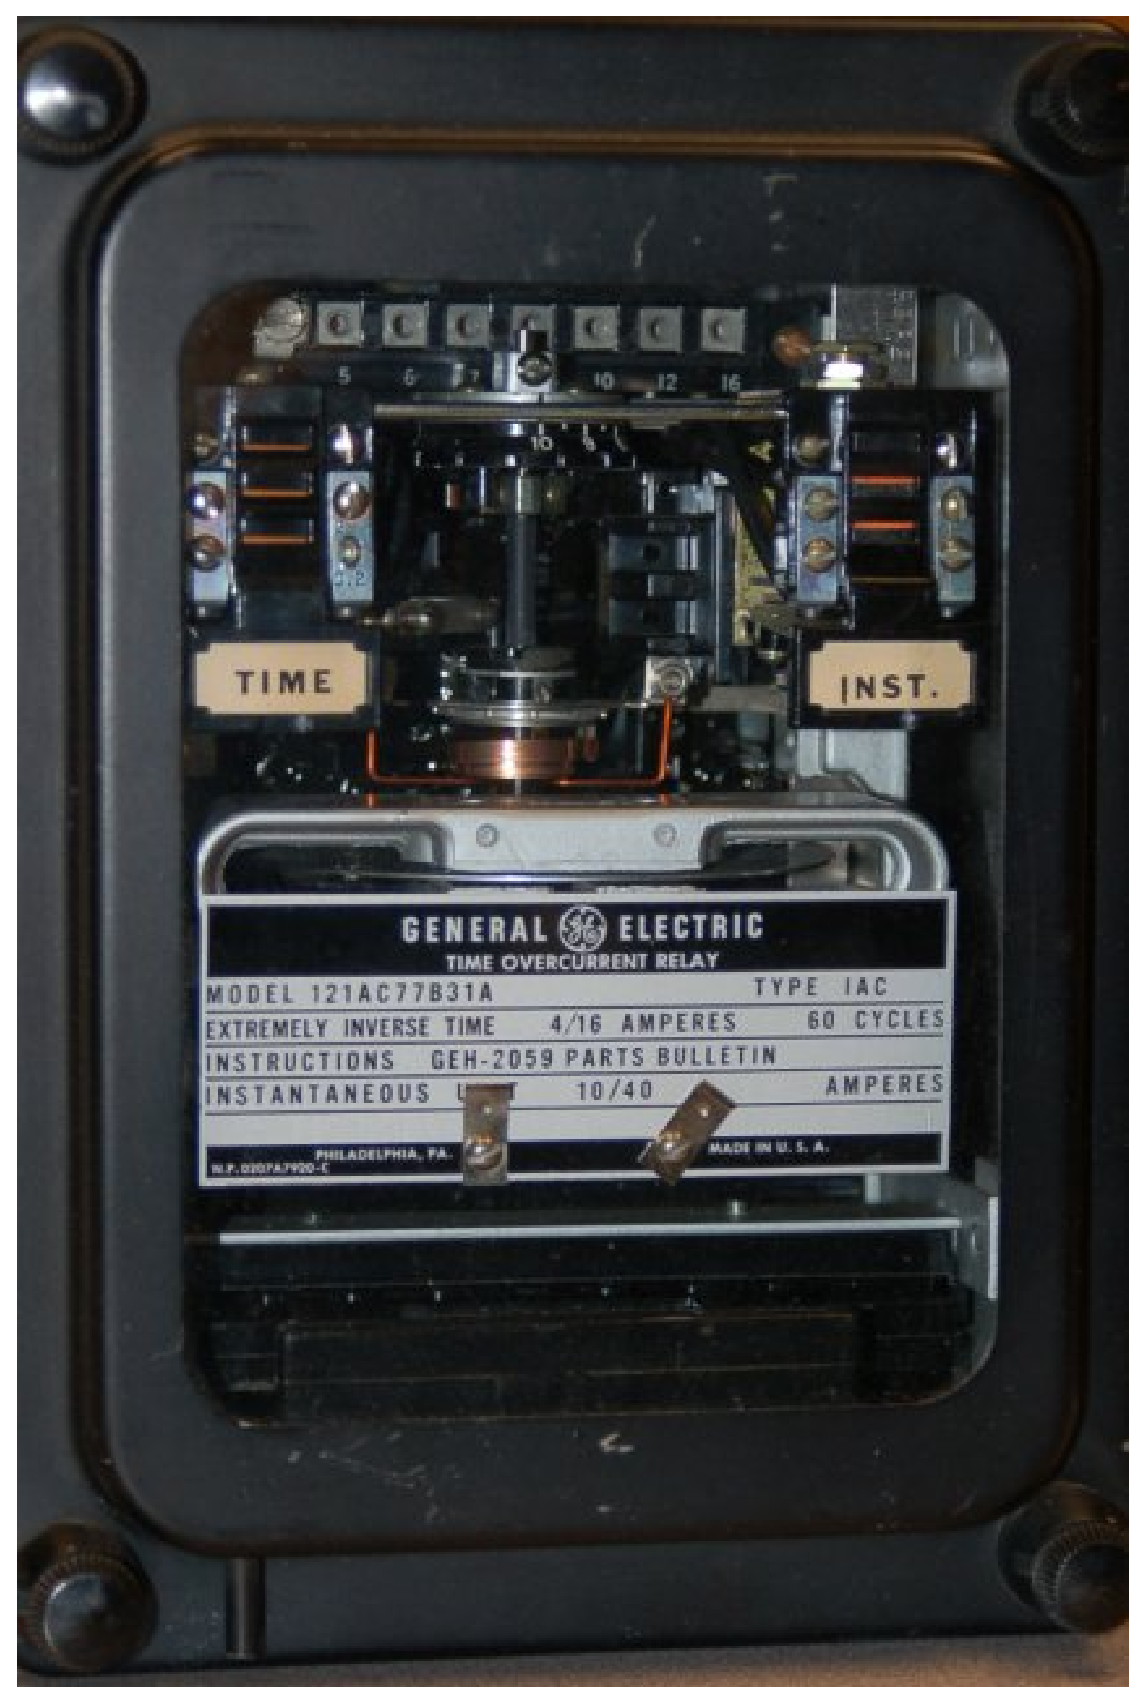
\includegraphics[width=15.5cm]{i01251x01.eps}$$

{\it Be very careful when handling one of these relays!  The induction disk shaft rests in two jeweled bearings, and may be damaged if the unit is dropped or the disk forcibly turned.  When you rotate the disk by hand, please use only your fingertips, and touch the disk very lightly!}

\vskip 10pt

Partner with your classmates to drive current into the CT terminals of a time-overcurrent relay using a {\it relay test set} or some other suitable source of adjustable alternating current.  Apply slightly more current to the relay than what the tap setting is set for, and measure the trip contact status using a multimeter.  Ask your instructor for assistance with the relay test set, as it is capable of generating significant AC voltage and current values for input into protective relays.

%\vskip 10pt

%You will find an instruction manual for the General Electric model IAC77 and IAC78 instantaneous/time-overcurrent relay units in your Instrumentation Reference file collection.

\vskip 20pt \vbox{\hrule \hbox{\strut \vrule{} {\bf Suggestions for Socratic discussion} \vrule} \hrule}

\begin{itemize}
\item{} Demonstrate how setting the ``time dial'' to different positions affects the time required for the 51 relay to trip.  Is a small time dial number or a large time dial number needed to make the relay more sensitive (i.e. trip sooner)?
\item{} Suppose you were to remove the drag magnet from a 51 relay.  How would the relay's behavior be altered as a result of this component loss?
\item{} Suppose you were to remove the restraint spring from a 51 relay (the spiral spring responsible for applying a restraining torque to the induction disk).  How would the relay's behavior be altered as a result of this component loss?
\end{itemize}

\underbar{file i01251}
%(END_QUESTION)





%(BEGIN_ANSWER)

Your instructor will have some electromechanical relays for you to inspect.

%(END_ANSWER)





%(BEGIN_NOTES)


%INDEX% Electric power systems: protective relays (time-overcurrent)
%INDEX% Protective relay: time-overcurrent (51)

%(END_NOTES)

